\documentclass{beamer}

\usepackage{minted}
\usepackage{hyperref}
\usepackage{graphicx}
\hypersetup{
    colorlinks=true,
    linkcolor=blue,
    filecolor=magenta,      
    urlcolor=blue,
}
\title{Android Root Detection Evasion}
\author[Roberto Castellotti]{Roberto Castellotti \\ {\small Supervised by: prof. Giovanni Lagorio}}
\institute{Università di Genova}
\date{2022}

\begin{document}

\frame{\titlepage}

\begin{frame}{fundamentals: Android}
    https://developer.android.com/guide/components/fundamentals 
\end{frame}

\begin{frame}{fundamentals: java to bytecode and back}
mobisec native code
\end{frame}

\begin{frame}{fundamentals: unlocking bootloader, recovery, root (con magisk)}
    lineage, magisk, twrp, tool vari approfondimento dm verity
    a cosa serve il root
\end{frame}


\begin{frame}{root detection: why}

\end{frame}


\begin{frame}[fragile]{root detection: how}

    \begin{itemize}
        \item check for root management apps (\texttt{com.topjohnwu.magisk})
\begin{minted}[fontsize=\footnotesize]{java}
import android.content.pm.PackageManager;
import android.content.Context;
private final Context mContext;
PackageManager pm = mContext.getPackageManager();
pm.getPackageInfo(packageName, 0);
\end{minted}
        \item check root cloaking appps {\small (\texttt{com.devadvance.rootcloak},\texttt{de.robv.android.xposed.installer})}
        \item check for dangerous applications (\texttt{com.dimonvideo.luckypatcher})
        \item check for binaries (\texttt{busybox,su})
\begin{minted}[fontsize=\footnotesize]{java}
File f = new File(path, filename);
boolean fileExists = f.exists();
\end{minted}
        \item check if some paths are writable (\texttt{/system, /sbin, /etc})
\begin{minted}[fontsize=\footnotesize]{java}
InputStream inputstream = Runtime.getRuntime().exec("mount")
\end{minted}
    \end{itemize}

\end{frame}

\begin{frame}{patch-and-reinstall}

    \begin{itemize}
        \item {\footnotesize \texttt{adb pull /data/com/app/com.package.name app.apk}}
        \item {\footnotesize \texttt{apktool d app.apk -output app}}
        \item patch
        \item {\footnotesize \texttt{apktool b app -output rebuilt-app.apk}}
        \item {\footnotesize \texttt{zipalign -f -p 4 rebuilt-app.apk  aligned-rebuilt-app.apk}}
        \item {\footnotesize \texttt{apksigner sign --ks ~/key.jks  aligned-rebuilt-app.apk}}
        \item {\footnotesize \texttt{adb install aligned-rebuilt-app.apk}}
        % well technically "this" approach needs it in order to pull the apk, but we can still obtain the apk using com.aurora.store
        \item this approach does not require the android device to be rooted 
    \end{itemize}

\end{frame}

\begin{frame}[fragile]{patch-and-reinstall: an example}

   The patching process is usually a matter of finding the methods performing root detection and patching them, here is an example from a popular financial services company's application:

\begin{figure}
    \centering 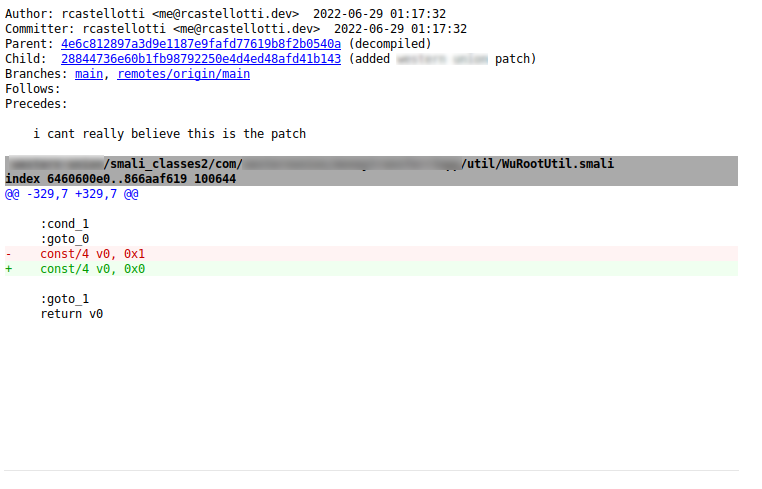
\includegraphics[scale=1.4]{patch.png}
    \caption{patching \mintinline{smali}{.method public static isDeviceRooted()Z} }
\end{figure}

\end{frame}


\begin{frame}{frida: a dynamic toolkit} 

    \begin{itemize}
        \item provides ability to inject scripts into black box processes.
        \item portable (Windows, macOS, GNU/Linux, iOS, Android)
        \item \textbf{injected mode}: \texttt{frida-server}: \texttt{frida-core} over TCP
        \item \texttt{frida-core}: a layer that packages up GumJS into a shared library that it injects into existing software, and provides a two-way communication channel for talking to your scripts.
        \item \textbf{on device:} {\footnotesize \texttt{./frida-server-15.1.27-android-arm64}}
        \item \textbf{on computer:} {\footnotesize \texttt{frida -U -l script.js -f com.package.name}}
        \item this approach could be better since it allows to patch applications without losing original package signature
    \end{itemize}
    
\end{frame}

\begin{frame}{tools used}

    \begin{itemize}
        \item \href{https://developer.android.com/studio}{Android Studio}
        \item \href{https://github.com/iBotPeaches/Apktool}{iBotPeaches/Apktool}:
        A tool for reverse engineering Android apk files
        \item \href{https://github.com/skylot/jadx}{skylot/jadx}: Dex to Java decompiler
        \item \href{https://github.com/scottyab/rootbeer}{scottyab/rootbeer}: Simple to use root checking Android library and sample app
    \end{itemize}
    
\end{frame}

\end{document}